%
% chapter.tex -- chapter 1, case study
%
% (c) 2024 Prof Dr Andreas Müller
%
\chapter{Eine Fallstudie: Wärme und Temperatur
\label{chapter:fallstudie}}
\kopflinks{Fallstudie: Wärme und Temperatur}
Eine oberflächliche Betrachtungsweise sieht in einem Feld, wie es in
der Physik in mannigfacher Weise vorkommt, nur eine reell- oder
vektorwertige Funktion.
Damit eine solche Funktion aber sinnvoll ein physikalisches Phänomen
beschreiben kann, müssen viele weitere Eigenschaften geklärt werden.
Zum Beispiel dürfen beobachtbare Grössen niemals von der Wahl des
Koordinatensystems abhängen.
Die Bewegungsgleichungen des Feldes oder Wirkung des Feldes auf
andere Körper müssen daher auf eine Art formuliert werden, dass sich
bei abweichender Wahl der Koordinaten die gleichen Effekte ergeben.
Man kann daher ein Feld nicht isoliert als Funktion betrachten.

In diesem Kapitel wird der Versuch unternommen, am Beispiel des
Temperaturfeldes und anderer intuitiv vertrauter Felder einige
Forderungen zusammenzutragen, die an physikalisch sinnvolle mathematische
Feldbegriffe gestellt werden müssen.
Sie sollen als Inspiration für die detaillierte Entwicklung der
Theorie in späteren Kapiteln dienen.

%
% 1-temperatur.tex
%
% (c) 2024 Prof Dr Andreas Müller
%

%
% Temperatur
%
\section{Temperatur
\label{buch:fallstudie:temperatur}}
\kopfrechts{Temperatur}
Die Temperatur ist eine Grösse, die ausdrückt, wie warm oder kalt ein
physikalisches ist.
\index{Temperatur}%
Die wichtigste Eigenschaft der Temperatur ist zweifellos, dass sie
sich zwischen sich in Kontakt befindlichen Körpern ausgleicht.
Wird ein heisser Körper mit einem kalten Körper in Berührung gebracht,
beginnt sich die Temperatur auszugleichen.
Zwei Körper haben genau die gleiche Temperatur, wenn sie längere
Zeit in Kontakt waren und sich die Temperaturen angleichen konnten.

Diese Eigenschaft reicht bereits aus, verschiedene zunächst willkürliche
Temperaturskalen zu definieren.
Zum Beispiel beobachtet man, dass sich ein Gas bei gleichem Umgebungsdruck
ausdehnt, wenn die Temperatur erhöht wird.
\index{Druck}%
Das Ausmass der Ausdehnung kann als Mass für die Temperatur verwendet
werden.
Ähnlich kann auch die Ausdehnung von Quecksilber in einer Glaskapillare
verwendet werden.
\index{Thermometer}%
\index{Quecksilber}%
Teilt man die Ausdehnung zwischen der Temperatur gefrierenden Wassers und
siedenden Wassers in 100 gleiche Teile, erhält man die Celsius-Temperaturskala.
Allerdings zeigt sich bei genauer Messung, dass die Ausdehnung von
\index{Celsius}%
Quecksilber nicht genau linear ist, so dass sich eine kleine Abweichung
von einem auf der Ausdehnung eines Gases basierenden Thermometer
ergibt.

Da die Temperatur nach obiger Definition nur durch Temperaturausgleich
gemessen werden kann, wird die Messung durch die Wärmekapazität des
Messgeräts beeinflusst.
Hat das Messgerät stark abweichende Temperatur, ändert sich die Temperatur
des zu messenden Körpers durch Kontakt sehr stark.
Eine sinnvolle Temperaturangabe ist damit nicht mehr möglich.
Der technische Fortschritt hat in der Vergangenheit aber ermöglicht, sehr
kleine Temperatursensoren zu konstruieren.
Heutzutage enthalten sogar Mikrochips wie Computerprozessoren spezielle
Dioden, die dazu da sind, die Temperatur des Chips zu überwachen und damit
den Chip vor Überhitzung zu schützen.
Wir nehmen daher im folgenden idealisierend an, dass die Temperatur beliebig
kleiner Teilkörper genügend genau gemessen werden kann.

%
% Das Temperaturfeld
%
\subsection{Das Temperaturfeld}
Der Ausgleich der Temperatur braucht Zeit.
Haben verschiedene Teile eines Körpers verschiedene Temperatur, dann
werden diese Unterschiede mit der Zeit zwar kleiner werden, aber je
kleiner die Unterschiede sind, desto langsamer wird auch der Ausgleich sein.
Die Temperatur eines Körpers ist daher eine Idealisierung, die nur
nach sehr langer Wartezeit erreicht werden kann.
Genau genommen ist die Temperatur eines Körpers notwendigerweise eine
Funktion $T(t,x,y,z)$, die sowohl von der Zeit wie auch von den
Ortskoordinaten abhängt.
Wir nennen sie für die Zwecke dieses Kapitels das {\em Temperaturfeld}.
\index{Temperaturfeld}%
Das Temperaturfeld eines isolierten Körpers konvergiert für
$t\to\infty$ gegen die ideale Temperatur des Körpers.

%
% Lokalität und Ableitungen
%
\subsection{Lokalität und Ableitungen}
In der Thermodynamik wird ausserdem gelehrt, dass die Temperatur die
\index{Thermodynamik}%
mittlere kinetische Energie der Atome oder Moleküle des Körpers wiedergibt.
Die statistische Mechanik untersucht, wie sich die kinetische Energie
zwischen verschiedenen Teilchen durch Stösse ausgleicht, bis sich eine
stationäre Verteilung einstellt.
Aus diesem Mechanismus kann man sofort schliessen, dass der
Temperaturausgleich ein {\em lokales} Phänomen ist.
\index{lokal}%
Stellt man in einem Medium an zwei verschiedenen Punkten verschiedene
Temperaturen fest, kann sich die Temperatur nur ausgleichen, wenn
sich auch die Temperatur an allen Punkten zwischen diesen beiden
ausgleicht.
Die Gleichungen, die die Veränderung der Temperatur in einem Punkt
mit der Zeit beschreiben, dürfen also nur die Information verwenden,
die sich aus dem Temperaturfeld an diesem Punkt ableiten lässt.
Nehmen wir an, dass die Funktion sich in einem Punkt in eine konvergente
Taylor-Reihe entwickeln lässt, dann kann man
\index{Taylor-Reihe}%
\[
T(t,x)
=
T(t,x_0) + DT(t,x_0)\, (x-x_0) + \frac{1}{2!} D^2T(t,x_0)(x-x_0,x-x_0) + \dots
\]
schreiben.
Die Ableitungen\footnote{Die Notation für die Ableitungen wird
in späteren Kapiteln definiert und erklärt, für die aktuelle Diskussion
kann sich der mit der Notation nicht vertraute Leser mit dem eindimensionalen
Fall $D^1f(x) = f'(x)$, $D^2f(x) = f''(x)$ oder $D^kf(x)=f^{(k)}(x)$ behelfen.}
\[
T(t,x_0), \quad
DT(t,x_0), \quad
D^2(t,x_0),\quad \dots\quad
D^k(t,x_0),\quad\dots
\]
sind Grössen, die nur von der Temperatur in einer beliebig kleinen
Umgebung des Punktes $x_0$ abhängen.
Es bleibt die offene Frage, ob sich auch noch weitere Grössen finden lassen.

\begin{aufgabe}
Es muss eine Theorie der lokalen Operatoren entwickelt werden, mit deren
Naturgesetze formuliert werden können.
Die Theorie muss den klassischen Begriff der Ableitung umfassen.
\end{aufgabe}

Die Geschwindigkeit, mit der sich die Temperatur in einem Punkt
an die Temperatur der näheren Umgebung anpasst, hängt von den
Ableitungen in diesem Punkt ab.
Die Zeitableitung von $T$ muss daher eine Funktion der Ableitungen
sein.
Die Zeitentwicklungsgleichung muss daher eine Differentialgleichung
der Form
\begin{equation}
\frac{\partial T}{\partial t}
=
F\biggl(x,
T,
\frac{\partial T}{\partial x},
\frac{\partial^2 T}{\partial x^2},
\dots
\biggr)
\label{buch:fallstudie:eqn:allgwaermeleitung}
\end{equation}
sein.

%
% Symmetrien
%
\subsection{Symmetrien}
Es gibt keine experimentellen Anzeichen, dass die Wärmeausbreitung
eine Richtung bevorzugt.
\index{Symmetrie}%
Die Differentialgleichung
\eqref{buch:fallstudie:eqn:allgwaermeleitung}
muss daher bei einer Spiegelung $x\mapsto -x$ unverändert bleiben.
Bei einer solchen Spiegelung ändern die ungeraden Ableitungen
das Vorzeichen, die Funktion $F$ muss daher gerade in den Argumenten
für die ungeraden Ableitungen sein.
In der einfachsten Form einer Wärmeleitungsgleichung ist die rechte
Seite der Gleichung \eqref{buch:fallstudie:eqn:allgwaermeleitung}
eine Funktion nur von $x$ und der zweiten Ableitung von $T$, die
ersten Ableitungen dürfen nicht vorkommen.

%
% Die Wärmeleitungsgleichung
%
\subsection{Die Wärmeleitungsgleichung}
Aus Experimenten weiss man aber auch, dass die Geschwindigkeit der
Temperaturänderung proportional ist zur Temperaturdifferenz.
Die Temperaturänderungsrate im Punkt $x$, die von der Temperaturdifferenz
zum benachbarten Punkt $x+h$ verursacht wird, ist daher
\begin{align*}
\biggl(\frac{\partial T}{\partial t}\biggr)_{\text{rechts}}
&=
a(h) (T(x+h)-T(x))
\intertext{für eine geeignete, von $h$ abhängige Proportionalitätskonstante
$a(h)$.
Die vom linken Nachbarpunkt beigesteuerte Änderungsrate ist}
\biggl(\frac{\partial T}{\partial t}\biggr)_{\text{links}}
&=
a(h) (T(x-h)-T(x))
\intertext{Die gesamte Änderungsrate ist daher}
\frac{\partial T}{\partial t}
&=
a(h) \bigl(T(x+h) - 2T(x) + T(x-h)\bigr).
\end{align*}
Wenn die Temperaturdifferenzen zu den Nachbarpunkten gleich gross 
sind, verschwindet die Änderungsrate.
Sie kann daher nur von der zweiten Ableitung abhängen.
Der Faktor $a(h)$ muss so gewählt werden, dass im Grenzwert
\[
\lim_{h\to 0}
a(h) \bigl( T(x+h)-2T(x)+T(x-h)\bigr)
=
a_0
\frac{\partial T^2}{\partial x^2}
\]
ein Vielfaches der zweiten Ableitung entsteht.
Damit ist die eindimensionale Wärmeleitungsgleichung
\index{Warmeleitungsgleichung@Wärmeleitungsgleichung}%
\begin{equation}
\frac{\partial T}{\partial t}
=
\kappa \frac{\partial^2 T}{\partial x^2}
\label{buch:fallstudie:waermeleitungsgleichung}
\end{equation}
gefunden.
Für beliebige Dimension ist die zweite Ableitung auf der rechten
Seite durch den Laplace-Operator
\index{Laplace-Operator}%
\[
\Delta T
=
\frac{\partial^2 T}{\partial x_1^2}
+\dots+
\frac{\partial^2 T}{\partial x_n^2}
\]
zu ersetzen.

%
% Wohldefinierte Lösungen
%
\subsection{Wohldefinierte Lösungen}
Die Verwendung der Ableitungen führt jedoch auf ein anderes Problem.
Die statistische Theorie der Wärmelehre erklärt auch, dass die Temperatur
ein einem kleinen Teil eines Körpers zufälligen Fluktuationen unterworfen
ist, die umso grösser werden können, je kleiner der Teil ist.
Die Ableitung ist der Grenzwert der Differenzenquotienten
\[
\lim_{s\to 0}
\frac{T(x_0+s\Delta x) - T(x_0)}{s}.
\]
Die Differenz im Zähler wird aber für für kleiner werdendes $s$ immer
weniger sinnvoll.
Die Verwendung der Ableitung ist daher ebenfalls eine Idealisierung.
Die Bewegungsgleichungen für das Temperaturfeld müssen daher von einer
Art sein, dass ein Störung des Feldes um kleine Fluktuationen nicht
zu einer gänzlich anderen Lösung führen.

Ein chaotisches dynamisches System wie das Lorenz-System zeichnet sich
dadurch aus, dass unmessbar kleine Unterschiede in den Anfangsbedingungen,
die zum Beispiel durch statistische Fluktuationen verursacht sein können,
zu verschiedenen Lösungen führen können.
\index{Chaos}%
Das Verhalten des Feldes wird damit für alle praktischen Zwecke nicht
vorhersagbar.
Die Wärmeleitungsgleichung hat jedoch die interessante mathematische
Eigenschaft, dass Sie einem Maximumprinzip gehorcht.
\index{Maximumprinzip}%
Es besagt, dass die extreme Werte in einem Teil des Randes des Körpers
sich sofort ausgleichen und die Lösung der Wärmeleitungsgleichung
mindestens für kurze Zeiten nur Werte hat, die kleiner sind als die 
Extremwerte zu Beginn.

Das Problem, dass das Feld nicht exakt bestimmt werden kann, gefährdet
nicht nur beim Temperaturfeld die Vorhersagbarkeit.
Auch bei Strömungsfeldern, die von den nichtlinearen
Navier-Stokes-Gleichungen beschrieben werden, muss eine solche
\index{Navier-Stokes-Gleichung}%
Stabilitätseigenschaft mindestens für kurze Zeit weiterhin gelten,
wenn die Theorie überhaupt testbare Vorhersagen ermöglich soll.
Die Bewegungsgleichung einer erfolgreichen Feldtheorie müssen daher
von einer Art sein, die die Existenz und Eindeutigkeit von Lösungen
mindestens für kurze Zeit und ein kleines Raumgebiet garantieren.

%
% Wärmeleitfähigkeit
%
\subsection{Wärmeleitfähigkeit}
Die Masseinheiten der beiden Seiten der Wärmeleitungsgleichung 
\eqref{buch:fallstudie:waermeleitungsgleichung}
sind
\[
\biggl[
\frac{\partial T}{\partial t}
\biggr]
=
\biggl[
\frac{\text{K}}{\text{s}}
\biggr]
=
[\kappa]
\biggl[
\frac{\partial^2 T}{\partial x^2}
\biggr]
=
[\kappa]
\biggl[
\frac{\text{K}}{\text{m}^2}
\biggr].
\]
Es folgt, dass die Masseinheit der Wärmeleitfähigkeit $\kappa$
\index{Warmeleitfahigkeit@Wärmeleitfähigkeit}%
\index{kappa@$\kappa$}%
\[
[\kappa]
=
\biggl[
\frac{\text{s}}{\text{m}^2}
\biggr]
\]
keine absolute Grösse ist.
Sie hängt vom für die Zeit- und die Raumdimensionen gewählten
Koordinatensystem ab.
Es ist daher zu ermitteln, wie sich $\kappa$ zusammen mit den
Differentialoperatoren verändert, wenn das Koordinatensystem
geändert wird.

\begin{aufgabe}
Es ist eine Theorie der Differentialoperatoren zu entwickeln, die
unabhängig vom Koordinatensystem formuliert werden kann.
\end{aufgabe}


%
% 2-waermekapazitaet.tex
%
% (c) 2024 Prof Dr Andreas Müller
%

%
% Wärmekapazität
%
\section{Wärmekapazität
\label{buch:fallstudie:waermekapazitaet}}
\kopfrechts{Wärmekapazität}
Wie schon angedeutet ist die Temperatur $T$ ein Mass für die im Körper
vorhandene kinetische Energie $U$.
\index{kinetische Energie}%
Für kleine Temperaturdifferenzen kann man zunächst annehmen, dass
es einen linearen Zusammenhang zwischen Energie und Temperatur gibt.
Die Steigung 
\[
C
=
\frac{\partial U}{\partial T}
\]
heisst die {\em Wärmekapazität} des Körpers.
\index{Warmekapazitat@Wärmekapazität}%

Je mehr Material zur Verfügung steht, desto grösser ist auch die Energie,
die bei einem Körper gespeichert werden kann.
Die Lokalität suggeriert, dass sich die Gesamtenergie eines Körpers 
\index{Lokalitat@Lokalität}
additiv aus den Energiemengenn der einzelnen Teile zusammensetzt.
Teilt man durch die Masse eines solchen kleinen Teils, erhält man die
spezifische Wärmekapazität $c$.
Sie ist eine Eigenschaft des Materials, aus dem das Teil besteht,
und hängt nicht mehr von der Grösse des Körpers ab.
Es ist aber möglich, dass $c$ von weiteren Grössen wie dem Druck oder der
chemischen Zusammensetzung abhängt, die nicht homogen sein muss.
Insbesondere kann $c$ wieder eine Funktion der Raumkoordinaten sein.

Multipliziert man $c(x)$ mit der Dichte $\varrho(x)$ des Materials,
\index{Dichte}%
entsteht eine Grösse, mit der sich aus der Temperatur sofort die
Dichte der gespeicherten Energie berechnen lässt.
In einem gewählten Koordinatensystem mit den Koordinaten $(x_1,\dots,x_n)$
wird daher bekannt sein, wie gross das Volumen eines kleinen
Quaders mit Kantenlängen $\Delta x_1$, $\Delta x_2$ und $\Delta x_3$ 
bestimmt werden kann.
Schreiben wir $v(x) \Delta x_1\,\Delta x_2\,\Delta x_3$ für dieses 
Volumen, wird der Energieinhalt durch das Volumenintegral
\[
U
=
\int_V T(x) c(x)\varrho(x) v(x)\,dx_1\,dx_2\,dx_3
\]
gegeben.
Während die Faktoren $T(x) c(x) \varrho(x)$ nicht von der Wahl der
Koordinaten abhängt, hängt die Funktion $v(x)$ vom Koordinatensystem
ab.

\begin{aufgabe}
Die Theorie der Integration ist so zu formulieren, dass automatisch
sichergestellt ist, dass ein Koordinatenwechsel die mit dem Integralbegriff
formulierten Gesetzmässigkeiten nicht verändert.
\end{aufgabe}


%
% 3-waermefluss.tex
%
% (c) 2024 Prof Dr Andreas Müller
%

%
% Wärmefluss
%
\section{Wärmefluss
\label{buch:fallstudie:waermefluss}}
\kopfrechts{Wärmefluss}
Betrachtet man einen von einer geschlossenen Fläche $S$ berandetes
Volumen in einem Körper, dann bewirken Temperaturunterschiede zwischen
Teilen des Körpers auf eiden Seiten der Fläche $S$, dass Wärme durch
die Fläche fliessen.
Der Gradient
\[
\operatorname{grad} T(x)
=
\nabla T
=
\renewcommand{\arraystretch}{1.9}
\begin{pmatrix}
\displaystyle \frac{\partial T}{\partial x_1}\\
\displaystyle \frac{\partial T}{\partial x_2}\\
\displaystyle \frac{\partial T}{\partial x_3}
\end{pmatrix}
\]
beschreibt die Richtung der grössten Temperaturzunahme.
Unterschieden sich zwei Punkte um den Vektor $\vec{v}$, dann ist der
Temperaturunterschied in erster Näherung gegeben durch das Skalarprodukt
$\vec{v}\cdot \nabla T$.
Sofern der Gradient parallel zur Fläche $S$ ist, kann keine Energie
durch die Fläche fliessen und die Energie im Inneren von $S$
ist erhalten.

Ist $\vec{n}$ in jedem Punkt der Fläche ein Vektor, der senkrecht
auf der Fläche steht, dann ist $\vec{n}\cdot \nabla T$ proportional
zum Wärmefluss.
Um den Energieverlust oder -gewinn durch die Fläche $S$ zu
berechnen, muss ein Integralbegriff konstruiert werden, der
nur vom Gradienten $\nabla T$ und der Oberfläche $S$ abhängt.
Die Parametrisierung der Oberfläche darf dabei genausowenig einen
Einfluss haben wie die Wahl des Koordinatensystems, mit dem der
Gradientvektor berechnet wird.

Ein weiteres Beispiel ist aus der Mechanik bekannt.
Das Gravitationsfeld $\smash{\vec{F}}$ als Vektorfeld kann als
Gradient $\smash{\vec{F}}=\nabla\varphi$ des Gravitationspotenials
$\varphi$ gefunden werden.
Die Arbeit, die zwischen den Punkten $A$ und $B$ geleistet
wird, wird durch das Integral
\[
W
=
\int_A^B \vec{F}\cdot d\vec{s}
=
\int_A^B \nabla \varphi \cdot d\vec{s}
\]
unabhängig vom gewählten Weg berechnet.
Auch in diesem Fall ist eine zentrale physikalische Grösse durch
ein Integral von Funktionen und Ableitungen gegeben, welches über
eine in diesem Fall eindimnensionale Untermannigfaltigkeit 
erstreckt wird.
Sowohl die Ableitungen wie auch die Parametrisierung des Weges
sind koordinatenabhängig.

\begin{aufgabe}
Konstruiere eine koordinatenunabhängige Theorie der Integration
von Funktioenn und Ableitungen auf beliebigen Untermannigfaltigkeiten
des Raumes und Sätze, die Bilanzbeziehungen wie die Energieerhaltung
beim Fluss Wärmeenergiefluss durch eine Oberfläche zu formulieren
erlauben.
\end{aufgabe}


%
% 4-prinzipal.tex
%
% (c) 2024 Prof Dr Andreas Müller
%

%
% Prinzipalbündel
%
\section{Zusammenhang und Prinzipalbündel
\label{buch:fallstudie:prinzipalbuendel}}
Es gibt Vektorfelder, die nichts mit den Verschiebungsvektoren im
Definitionsbereich zu tun haben.
Ein Farbbild ordnet jedem Punkt der Bildebene einen dreidimensionalen
Vektor zu, der die Farbkomponenten $R$, $G$ und $B$ enthält.
In diesem Fall ist klar, dass die Verschiebung oder Drehung in der
Bildebene sich nicht auf die Farben auswirkt.

Auch die elektrischen und magnetischen Feldvektoren werden zwar
oft im gleichen Raum dargestellt, haben aber eigentlich nur indirekt
etwas mit den Raumdimensionen zu tun.
Aus dem elektrischen Feldvektor lässt sich durch Multiplikation die
Kraft berechnen, die das elektrische Feld auf eine Testladung ausübt,
die sich in Form der Beschleunigung der Ladung und der Krümmung der
Bahnkurve bemerkbar macht.
Es stellt sich aber spätestens in der speziellen Relativitätstheorie
heraus, dass das elektrische Potential $\varphi$ und das Vektorpotential
$\vec{A}$ die geeigneteren Grössen zur Beschreibung des elektromagnetischen
Feldes sind.
Die sogenannten Eichtransformationen sind zusätzliche Symmetrien, denen
das aus $\varphi$ und $\vec{A}$ kombinierte genügt.
Sie können interpretiert werden als eine Modifikation der
Ableitungsoperatoren, die ihrerseits mit den Verschiebungsvektoren
verbunden sind.

Auf gekrümmten Flächen ist es nicht selbstverständlich, einen
Tangentialvektor in einem Punkt mit einem Tangentialvektor in einem
Nachbarpunkt zu vergleichen.
Der Transport entlang einer Kurve in einer gekürmmten Fläche wirkt
sich daher auch auf den Transport von Tangentialvektoren aus.
Dies wirkt sich auf den Begriff der Ableitung aus.
Für den Vergleich ist ein sogenannter {\em Zusammenhang} notwendig, mit
dem sich die {\em kovariante Ableitung} konstruieren lässt.
Ein ähnliches Phänomen tritt bei der Beschreibung von Strömungen
auf, wo Vektoren von der Strömung transportiert werden und dabei
verändert werden können.

%
% spin12.tex
%
% (c) 2024 Prof Dr Andreas Müller
%
\begin{figure}
\centering
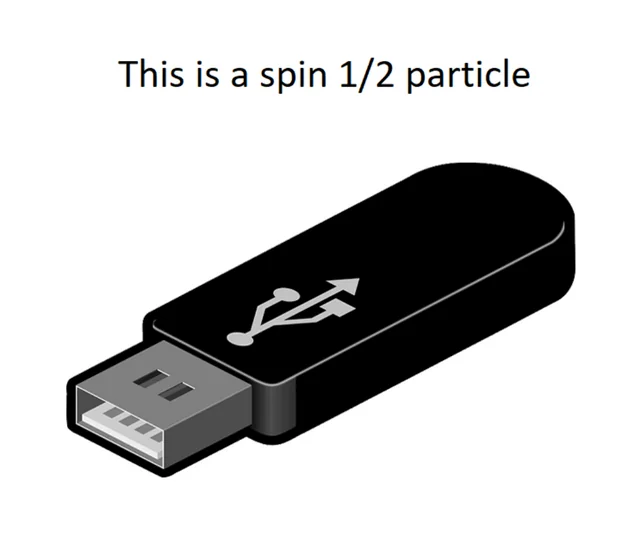
\includegraphics[width=8cm]{chapters/010-fallstudie/images/spin12.png}
\caption{Internet Meme, welches die frustrierende Erfahrung, dass sich
ein USB-Stick oft erst beim dritten oder vierten Versuch einstecken
lässt, scherzhaft als Spin-$\frac12$-Phänomen interpretiert.
\label{buch:fallstudie:fig:spin12}}
\end{figure}
%

Der Spin eines Elektrons ist eine Quanteneigenschaft, die mit der
Drehung des Raums gekoppelt ist.
Da ein Elektron zwei mögliche Spin-Orientierungen haben kann, hat
die Wellenfunktion einen zweidimensionalen komplexen Vektor als Wert.
Die speziellen unitären Matrizen der Gruppe $\operatorname{SU}(2)$ 
operieren auf diesen Vektoren.
Ausserdem lässt sich zeigen, dass zu jeder Matrix in $\operatorname{SU}(2)$
eine Drehung des dreidimensionalen Raumes mit einem Element der
Gruppe $\operatorname{SO}(3)$ gehört.
Die ``Drehungen'' im zweidmensionalen Raum der Spinvektoren ist also
mit den Drehungen im dreidimensionalen Raum gekoppelt, wie dies auch
durch Internet-Memes wie jenes in Abbildung~\ref{buch:fallstudie:fig:spin12}
aufs Korn nehmen.
Die genannte Art von Kopplung wird durch ein {\em Prinzipalbündel}
abstrakt dargestellt.

\begin{aufgabe}
Die Theorie der Ableitung muss so erweitert werden dass sie auch für
Vektorfelder funktioniert, die nicht direkt mit Tangentialvektoren
verbunden werden können und die zusätzliche Symmetrieeigenschaften
haben.
\end{aufgabe}

Die Dirac-Gleichung ist eine Form der Wellengleichung für Elektronen,
die mit der speziellen Relativitätstheorie vereinbar ist.
Sie wurden 1928 von P.~A.~M.~Dirac entdeckt und beschreibt das Elektron
als eine Wellenfunktion mit Werten in einem vierdimensionalen komplexen
Vektorraum.
Zwei der Komponenten konnten unmittelbar als die beiden Spinkomponenten
identifiziert werden.
Die anderen beiden Komponenten interpretiert Dirac als ein Teilchen,
welches identische Eigenschaften wie ein Elektron aufweist, ausser dass
die Ladung entgegengesetzt ist.
Tatsächlich gelang es C.~D.~Anderson 1932, ein Teilchen mit diesen
Eigenschaften nachzuweisen, es wird heute das Positron genannt und ist
das Antiteilchen des Elektrons.







